\subsection{Logistic regression}
As first approach we tried to model our target using \textit{Logistic Regression}.

First of all we fitted a model using all the features, that we will name model A, and the result is displayed in \Fig~\ref{fig:LRAllSum}. The model suggested that many variables are not significantly different from zero, with respect to an $\alpha = 0.01$. Therefore we removed those variables and fitted the model again getting the one in \Fig~\ref{fig:LRImpSum}, that we will name model B.

\begin{figure}[h]
	\begin{subfigure}{.6\textwidth}
		\centering
		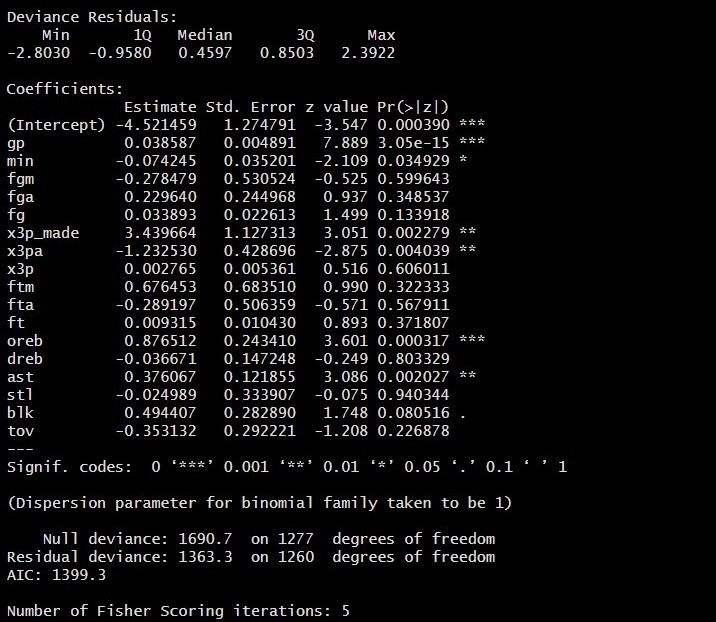
\includegraphics[width=0.7\linewidth]{ImageFiles/Classification/LogReg/log_reg_all_summary}
		\caption{Logistic Regression with all features.}
		\label{fig:LRAllSum}
	\end{subfigure}
	\begin{subfigure}{.6\textwidth}
		\centering
		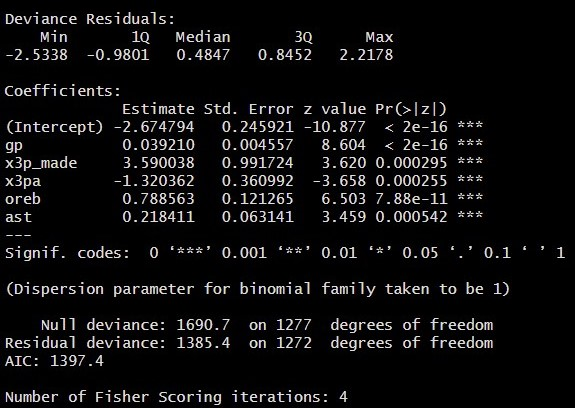
\includegraphics[width=0.8\linewidth]{ImageFiles/Classification/LogReg/log_reg_imp_summary}
		\caption{Logistic Regression with only significant features.}
		\label{fig:LRImpSum}
	\end{subfigure}
	\caption{Logistic Regression Model Summary.}
	\label{fig:LRSum}
\end{figure}

It can be observed that there is no significant change in performance. When all variables are used, the accuracy is $72.77\%$, compared to $71.36\%$ in the second case. Furthermore, the AIC coefficient changes from 1399.3 to 1397.3, which could be considered almost the same. 

Another comparison made by the two models is concerning the probabilities predicted since values close to 0.5 suggest high uncertainty of the model. \Fig~\ref{fig:ProbPred} shows as histograms the predicted values distribution for both models.

\begin{figure}[h]
	\begin{subfigure}{.6\textwidth}
		\centering
		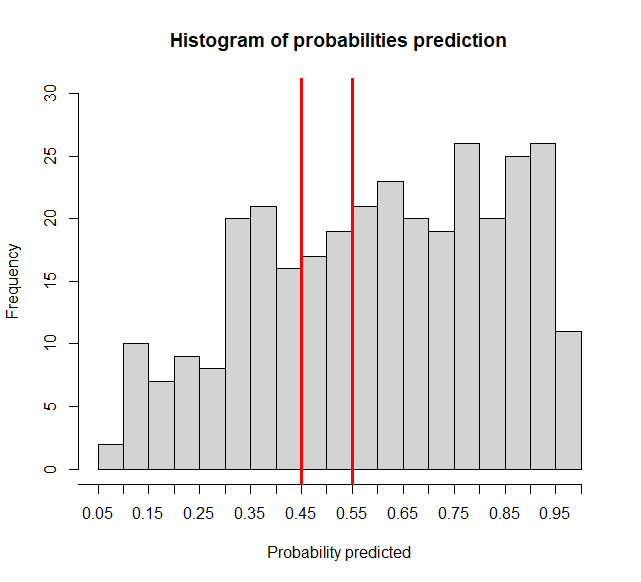
\includegraphics[width=0.7\linewidth]{ImageFiles/Classification/LogReg/probability_pred_all}
		\caption{Probabilities predicted by model A.}
		\label{fig:ProbPredA}
	\end{subfigure}
	\begin{subfigure}{.6\textwidth}
		\centering
		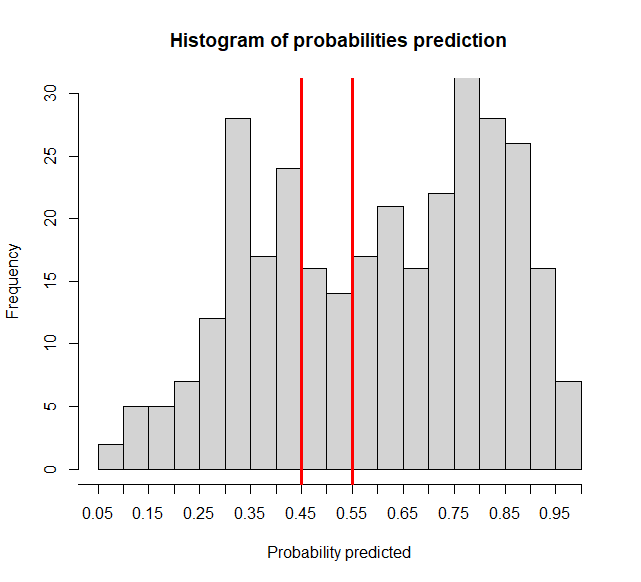
\includegraphics[width=0.7\linewidth]{ImageFiles/Classification/LogReg/probability_pred_imp}
		\caption{Probabilities predicted by model B.}
		\label{fig:ProbPredB}
	\end{subfigure}
	\caption{Probabilites predicted.}
	\label{fig:ProbPred}
\end{figure}
